
% TODO:
%    .append() with ignore_index=True
%     OR maybe just .reset_index(drop=True)   (more general purpose)
%
% memory diagrams, including .copy()

\chapter{Three kinds of aggregate data}

Now it's time to consider some loftier goals for our lowly atomic bits of data.
Most anything interesting in Data Science comes from arranging them together in
various ways to form more complex structures. This chapter is the subject of
these.

\index{aggregate data}
\section{Aggregate data types}

The number of ways in which pieces of data can be arranged is far greater than
the number of different atomic types. These various ways all have names, some
of them nerdy and/or exotic like ``hash tables,'' ``binary search trees,'' and
``skip lists.'' Nevertheless, there are again three basic ones which will form
the basis of our study: they're called \textbf{arrays}, \texttt{associative
arrays}, and \texttt{tables}. As before, we'll consider each one conceptually
first, and then look at how to use them in Python.

\index{array}
\subsection{Arrays}

An \textbf{array} is simply a sequence of items, all in a row. We call those
items the ``\textbf{elements}'' of the array. So an array could have ten whole
numbers as its elements, or a thousand strings of text, or a million real
numbers.

Normally, we will deal with \textbf{homogeneous} arrays, in which all the
elements are of the same type; this turns out to be what you want 99\% of the
time. Some languages (including Python) do permit creating a
\textbf{heterogeneous} array, which could hold (say) three whole numbers,
sixteen reals, and four strings of text all mixed together. But usually you're
using an array to contain a bunch of related values, like the current balances
of all the accounts in your bank, or the Twitter screen names of all a user's
followees.

Figure~\ref{fig:array} shows what those two examples would look like
conceptually. One has four strings of text, and the other five real numbers.
Note that each \textit{entire set} of elements is \textit{one} variable. We
might call the left one ``\texttt{followees}'' and the right one
``\texttt{balances}.''

\begin{figure}[ht]
\centering
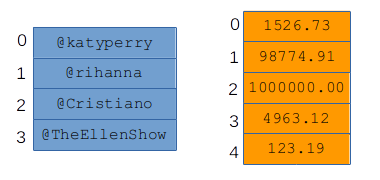
\includegraphics[width=0.6\textwidth]{array.png}
\caption{Two arrays.}
\label{fig:array}
\end{figure}

\index{index@index (pl:~indices)}
Worthy of special note are the numbers on the left-hand side. These numbers
are called the \textbf{indices} (singular:~\textbf{index}) of the array.
They exist simply so we have a way to talk about the individual elements. I
could say ``element \#2 of the \texttt{followees} array'' to refer to
\texttt{@Cristiano}.

\index{zero@zero, starting at}
And yes, you noticed that the index numbers start with 0, not 1. Yes, this is
weird. The reason I did that it is because nearly all programming languages
(including Python) number their array elements starting with zero, so you might
as well just start getting used to it now. It's really not hard once you get
past the initial weirdness.

Arrays are the most basic kind of aggregate data there is, and they are the
workhorse of a whole lot of Data Science processing. Sometimes they're called
\textbf{\texttt{list}s}, \textbf{\texttt{vector}s}, or
\textbf{\texttt{sequence}s}, by the way. (When a particular concept has lots of
different names, you know it's important.)

\subsection{Associative arrays}

\subsection{Data frames}

\section{The three kinds in Python}

\subsection{Arrays: \texttt{numpy}'s \texttt{ndarray}}

\subsection{Associative arrays: Python's \texttt{dict}}

\subsection{Data frames: \texttt{pandas}'s \texttt{DataFrame}}


% Somewhere: .map() for recoding
